\documentclass[tikz,border=0pt]{standalone}
\usepackage[T1]{fontenc}
\usepackage{helvet}
\renewcommand{\familydefault}{\sfdefault}
% Reuse accepted label-free artwork through vector viewports; no pixel editing.
\usepackage{graphicx}
\usetikzlibrary{arrows.meta,calc}
\tikzset{flow/.style={-{Stealth[length=1.6mm,width=1.1mm]},line width=.75pt},
 wirelabel/.style={fill=white,inner sep=1.2mm},
 every node/.style={font=\fontsize{9}{11}\selectfont,align=center,inner sep=1pt}}
% Arguments: source left/top/right/bottom pixels; destination left/bottom/width mm.
\newcommand{\artpiece}[7]{
 \pgfmathsetmacro{\pieceScale}{#7/((#3-#1)*.1)}
 \begin{scope}[shift={(#5,#6)},scale=\pieceScale,transform shape]
  \clip (0,0) rectangle ({(#3-#1)*.1},{(#4-#2)*.1});
  \node[anchor=south west,inner sep=0pt] at ({-#1*.1},{-(931-#4)*.1})
   {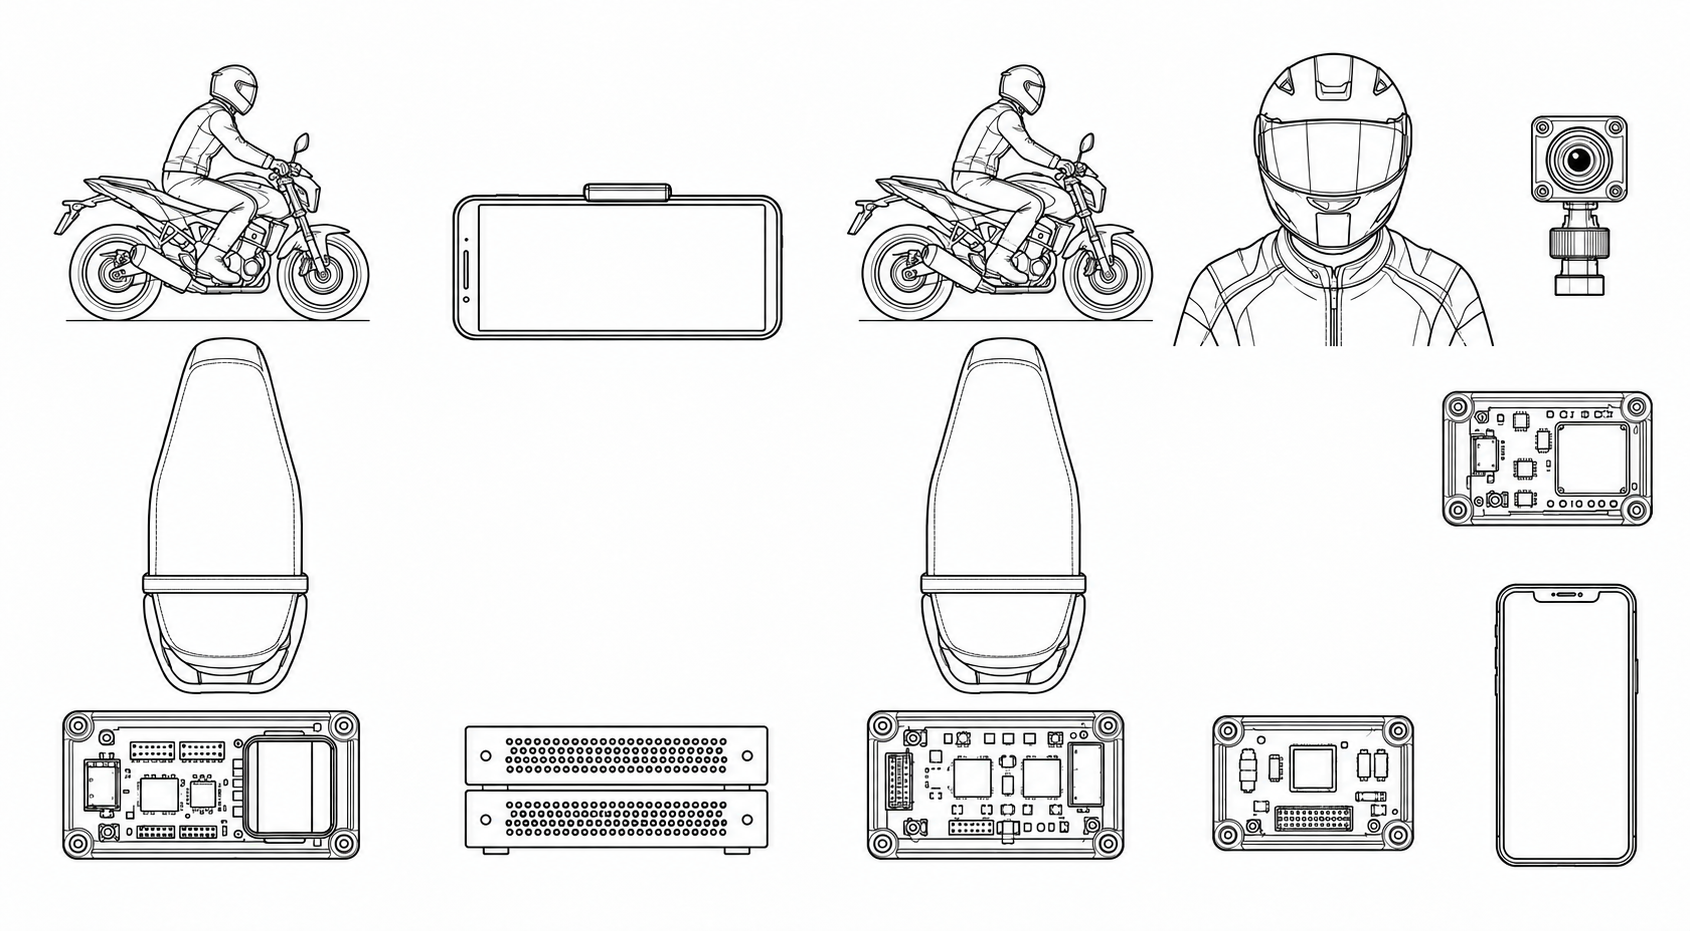
\includegraphics[width=169mm]{artwork-original.png}};
 \end{scope}}
\newcommand{\marker}[2]{
 \fill[white] (#1-2.4,#2-2.4) rectangle (#1+2.4,#2+2.4);
 \fill (#1-2,#2-2) rectangle (#1+2,#2+2);
 \fill[white] (#1-1.2,#2-1.2) rectangle (#1+1.2,#2+1.2);
 \fill (#1-1.2,#2-1.2) rectangle (#1,#2);
 \fill (#1,#2) rectangle (#1+1.2,#2+1.2);
}
\newcommand{\phoneglyph}[2]{
 \begin{scope}[shift={(#1,#2)}]
  \draw[densely dotted] (-8,0)--(8,0) (0,-13)--(0,13);
  \draw (0,10) .. controls (7,12) and (3,4) .. (7,-1)
    .. controls (11,-9) and (-4,-13) .. (-6,-7)
    .. controls (-9,0) and (-6,8) .. (0,10);
 \end{scope}}

\usetikzlibrary{patterns}
\tikzset{frameone/.style={line width=1.5pt,line join=miter,line cap=butt},frametwo/.style={line width=1pt,line join=miter,line cap=butt}}
\begin{document}
\begin{tikzpicture}[x=1mm,y=1mm,line width=.65pt,line cap=round,line join=miter]
\path[use as bounding box] (0,0) rectangle (240,180);

\draw[frameone] (3,91) rectangle (118,177) (122,91) rectangle (237,177);
\node[anchor=west] at (7,172) {A. Complementary posture sensing};
\artpiece{1170}{45}{1500}{345}{14}{119}{40}
\foreach \xx/\yy in {34/150.1,34/132.9,20.7/126.3,48.3/126.3}{\marker{\xx}{\yy}}
\artpiece{1520}{110}{1640}{302}{70}{135}{12}
\draw[dashed] (70,144)--(54,144);
\artpiece{1435}{384}{1660}{535}{90}{137}{20}
\draw[flow] (82,144)--(90,144);
\node[align=center] at (90,130) {Camera and\\Raspberry Pi};
\node[align=center] at (62,111) {4 camera-tracked reference markers:\\helmet top, chin and both shoulders};
\artpiece{130}{330}{315}{700}{22}{25}{25}
% Seat drawing used below in panel C; upper panel shows sensing grid abstractly.
\draw[frametwo] (70,157) rectangle (110,163);
\node at (90,160) {Optical branch};
\draw[frametwo] (14,95) rectangle (110,103);
\node at (62,99) {Relative positions describe head and torso orientation};
\node[anchor=west] at (126,172) {B. Bike Area Network: modular processing};
\draw[frametwo] (132,139) rectangle (174,159) (180,139) rectangle (222,159);
\node[align=center] at (153,149) {Pressure\\module};
\node[align=center] at (201,149) {Camera\\module};
\draw (153,139)--(153,128)--(201,128)--(201,139);
\draw[frametwo] (150,112) rectangle (204,124);
\node at (177,118) {Central Raspberry Pi};
\draw[flow] (177,128)--(177,124);
\node[wirelabel] at (177,134.5) {WebSockets};
\node[align=center] at (177,103) {Combine pressure distribution\\with head and shoulder geometry};
\draw[frameone] (3,23) rectangle (118,87) (122,23) rectangle (237,87);
\node[anchor=west] at (7,82) {C. Seat load distribution};
% Centered two-column, three-row sensor grid about the seat centerline.
\foreach \yy in {47,55,63}{\foreach \xx in {31.5,38.5}{\draw[fill=white] (\xx,\yy) circle (1.3);}}
\node[align=center] at (82,65) {6 force-sensitive\\resistors};
\node[align=center] at (82,50) {2 analog-to-digital\\converters};
\draw[flow] (47,51)--(58,51);
\node[align=center] at (82,35) {Pressure sensing\\Raspberry Pi};
\node[anchor=west] at (126,82) {D. Glanceable, contextual feedback};
\artpiece{1490}{580}{1645}{868}{132}{29}{23}
\begin{scope}[shift={(143.5,50)},scale=.7]\phoneglyph{0}{0}\end{scope}
\draw[dashed] (143.5,57) ellipse (4.8 and 7.5);
\draw (161,72)--(174,72);\node[anchor=west] at (178,72) {Current posture};
\draw[dashed] (161,65)--(174,65);\node[anchor=west] at (178,65) {Reference contour};
\node[align=left,anchor=west] at (162,52) {Forward/back and left/right lean\\Shoulder tilt and head stoop};
\node[align=left,anchor=west] at (162,35) {Interpret duration and ride history.\\Learning and full ride evaluation proposed.};
\draw[frameone] (3,3) rectangle (237,19);
\node[anchor=west,align=left] at (7,11) {Modules and feedback design reported.\\Contours are schematic, not measured riding results.};
\node[anchor=east,align=right] at (233,11) {Bagalkot and colleagues (2019), 443--450.\\Tangible, Embedded and Embodied Interaction; source: 445--449.\\Artwork: source-based conceptual reconstruction.};
\end{tikzpicture}
\end{document}
